%%%%%%%%%%%%%%%%%%%%%%%%%%%%%%%%%%%
% This is the LaTeX template for a Rutgers PhD or Masters Thesis
% Copyright J. A. Konkol 2023
% Distributed under LPPL 1.3 https://www.latex-project.org//lppl/
%%%%%%%%%%%%%%%%%%%%%%%%%%%%%%%%%%%

\documentclass[12pt,a4paper, oneside]{book}
\usepackage[utf8]{inputenc}
\usepackage{amsmath}
\usepackage{amsfonts}
\usepackage{amssymb}
%\usepackage[super,sort&compress,comma]{natbib}
\usepackage{rsc}
\usepackage{graphicx}
\usepackage[left=1.5in,right=1in,top=1in,bottom=1in]{geometry}
\usepackage{setspace}
\usepackage{fancyhdr}
\usepackage{url}
\def\UrlBreaks{\do\/\do-}
\usepackage{breakurl}
\usepackage[breaklinks]{hyperref}
\usepackage{titlesec}
\usepackage{xcolor}
\usepackage{ifthen}
\usepackage{siunitx}
\usepackage[version=4]{mhchem}
\usepackage{mciteplus}
\usepackage{booktabs}

%%%%%%%%%%%%%%%%%%%%%%%%%%%%%%%%%%%%%%%%%%%%
% Template specific packages
%%%%%%%%%%%%%%%%%%%%%%%%%%%%%%%%%%%%%%%%%%%%
\usepackage[CBE,PhD]{RUTitle}
\usepackage{RUCopy}
\usepackage{RUAbstract}
\usepackage{RUDedication}

%%%%%%%%%%%%%%%%%%%%%%%%%%%%%%%%%%%%%%%%%%%%
% These commands rename the list of figures, list of tables, and add double spacing
%%%%%%%%%%%%%%%%%%%%%%%%%%%%%%%%%%%%%%%%%%%%
\let\mtcontentsname\contentsname
\renewcommand\contentsname{\MakeUppercase\mtcontentsname}
\renewcommand{\listfigurename}{\MakeUppercase{List of Illustrations}}
\renewcommand{\listtablename}{\MakeUppercase{List of Tables}}
\doublespacing

%%%%%%%%%%%%%%%%%%%%%%%%%%%%%%%%%%%%%%%%%%%%
% These commands set the style for the chapter titles
%%%%%%%%%%%%%%%%%%%%%%%%%%%%%%%%%%%%%%%%%%%%
\definecolor{gray75}{gray}{0.75}
\newcommand{\hsp}{\hspace{20pt}}
\titlespacing*{\chapter}{0em}{0em}{0em}
\titleformat{\chapter}[hang]{\Huge\bfseries}{\thechapter\hsp{$\vert$}\hsp}{0pt}{\Huge\bfseries}

%%%%%%%%%%%%%%%%%%%%%%%%%%%%%%%%%%%%%%%%%%%%%%%%%%%%%%%%%%%%%%%%%%%%%%
% Author details section
%%%%%%%%%%%%%%%%
% Replace the following as appropriate
%%%%%%%%%%%%%%%%%%%%%%%%%%%%%%%%%%%%%%%%%%%%%%%%%%%%%%%%%%%%%%%%%%%%%%
\author{A Student}
\title{Very impressive work}
\graduationDate{June 2023}
\supervisor{A Professor}


%%%%%%%%%%%%%%%%%%%%%%%%%%%%%%%%%%%%%%%%%%%%%%%%%%%%%%%%%%%%%%%%%%%%%%
% Command section
%%%%%%%%%%%%%%%%
% In the follow section you may define new commands
% for your thesis. Some example commands are provided.
% An example for a new float is also provided
%%%%%%%%%%%%%%%%%%%%%%%%%%%%%%%%%%%%%%%%%%%%%%%%%%%%%%%%%%%%%%%%%%%%%%
\newcommand{\wavenumber}{cm$^{-1}$}
\newcommand{\syncCoords}[2]{$\Phi({#1}, {#2})$}%Command to automatically format synchronous coordinates
\newcommand{\asyncCoords}[2]{$\Psi({#1}, {#2})$}%Command to automatically format asynchronous coordinates

\usepackage{newfloat}

\DeclareFloatingEnvironment[
  fileext = los ,
  listname = {List of Schemes} ,
  name = Scheme
]{scheme}
\renewcommand{\listschemename}{\MakeUppercase{List of Schemes}}

%%%%%%%%%%%%%%%%%%%%%%%%%%%%%%%%%%%%%%%%%%%%%%%%%%%%%%%%%%%%%%%%%%%%%%
% Document section
%%%%%%%%%%%%%%%%
% The following section is where you place your content.
%%%%%%%%%%%%%%%%%%%%%%%%%%%%%%%%%%%%%%%%%%%%%%%%%%%%%%%%%%%%%%%%%%%%%%

\begin{document}

\pagestyle{plain}
\fancyhf{}
\renewcommand{\headrulewidth}{0pt}
\fancyfoot[C]{\thepage}

\frontmatter

%%%%%%%%%%%%%%%%%%%%%%%%%%%%%%%%%%%%%%%%%%%%%%%%%%%%%%%%%%%%%%%%%%%%%%
% Copyright page
%%%%%%%%%%%%%%%%
% Remove the command \copyrightPage if this is for a proposal.
%%%%%%%%%%%%%%%%%%%%%%%%%%%%%%%%%%%%%%%%%%%%%%%%%%%%%%%%%%%%%%%%%%%%%%
\copyrightPage

\maketitle

%%%%%%%%%%%%%%%%%%%%%%%%%%%%%%%%%%%%%%%%%%%%%%%%%%%%%%%%%%%%%%%%%%%%%%
% Abstract
%%%%%%%%%%%%%%%%
% Insert your abstract into the following. You may also provide a tex
% file containing the abstract using \input{}.
%%%%%%%%%%%%%%%%%%%%%%%%%%%%%%%%%%%%%%%%%%%%%%%%%%%%%%%%%%%%%%%%%%%%%%
\begin{abstract}
This is my abstract, here I give an overview of the contents and results.
\end{abstract}

%%%%%%%%%%%%%%%%%%%%%%%%%%%%%%%%%%%%%%%%%%%%%%%%%%%%%%%%%%%%%%%%%%%%%%
% Acknowledgements/Dedication
%%%%%%%%%%%%%%%%
% Feel free to remove these if you don't want them. Do not include
% if this is a proposal document.
%%%%%%%%%%%%%%%%%%%%%%%%%%%%%%%%%%%%%%%%%%%%%%%%%%%%%%%%%%%%%%%%%%%%%%
\begin{acknowledgments}
I acknowledge these people.
\end{acknowledgments}

\dedication{I dedicate this to}

%%%%%%%%%%%%%%%%%%%%%%%%%%%%%%%%%%%%%%%%%%%%%%%%%%%%%%%%%%%%%%%%%%%%%%
% Table of content 
%%%%%%%%%%%%%%%%
% The following commands at the list of illustrations, tables, and schemes
% to the table of contents. If adding a different float environment, use
% the schemes as an example
%%%%%%%%%%%%%%%%%%%%%%%%%%%%%%%%%%%%%%%%%%%%%%%%%%%%%%%%%%%%%%%%%%%%%%

\tableofcontents

\cleardoublepage
\phantomsection
\addcontentsline{toc}{chapter}{\listtablename}
\listoftables

\cleardoublepage
\phantomsection
\addcontentsline{toc}{chapter}{\listfigurename}
\listoffigures


\cleardoublepage
\phantomsection
\addcontentsline{toc}{chapter}{\listschemename}
\listofschemes


\mainmatter

%%%%%%%%%%%%%%%%%%%%%%%%%%%%%%%%%%%%%%%%%%%%%%%%%%%%%%%%%%%%%%%%%%%%%%
% Thesis content
%%%%%%%%%%%%%%%%
% This is where your thesis content goes. You should use separate .tex
% files using \include{}.
%%%%%%%%%%%%%%%%%%%%%%%%%%%%%%%%%%%%%%%%%%%%%%%%%%%%%%%%%%%%%%%%%%%%%%
\chapter{Introduction}

This is my introduction.\footnote{This is the first footnote}

\section{Underwater basket weaving}

Here is a short overview of underwater basket weaving.\footnote{This is the second footnote}

\subsection{Freshwater basket weaving}

This joke is wearing thin, so here's the difference between subsub-, sub-, and sections.\footnote{This is an extremely long footnote that where to goal is to see if the footnotes are doublespaced or singlespaced as required by university quidelines.}

\subsubsection{Lakes}
Notice that subsubsections are un-numbered and do not appear in the TOC.
\subsubsection{Rivers}
\subsubsection{Ponds}

\subsection{Saltwater basket weaving}

\section{Open questions}

Here is a short section on gaps in the literature for underwater basket weaving.

\chapter{Methods}

Whatever my methods, I need to keep in mind the importance of reproducibility.\cite{Sholl2019}

\begin{figure}[htbp]
	\centering
	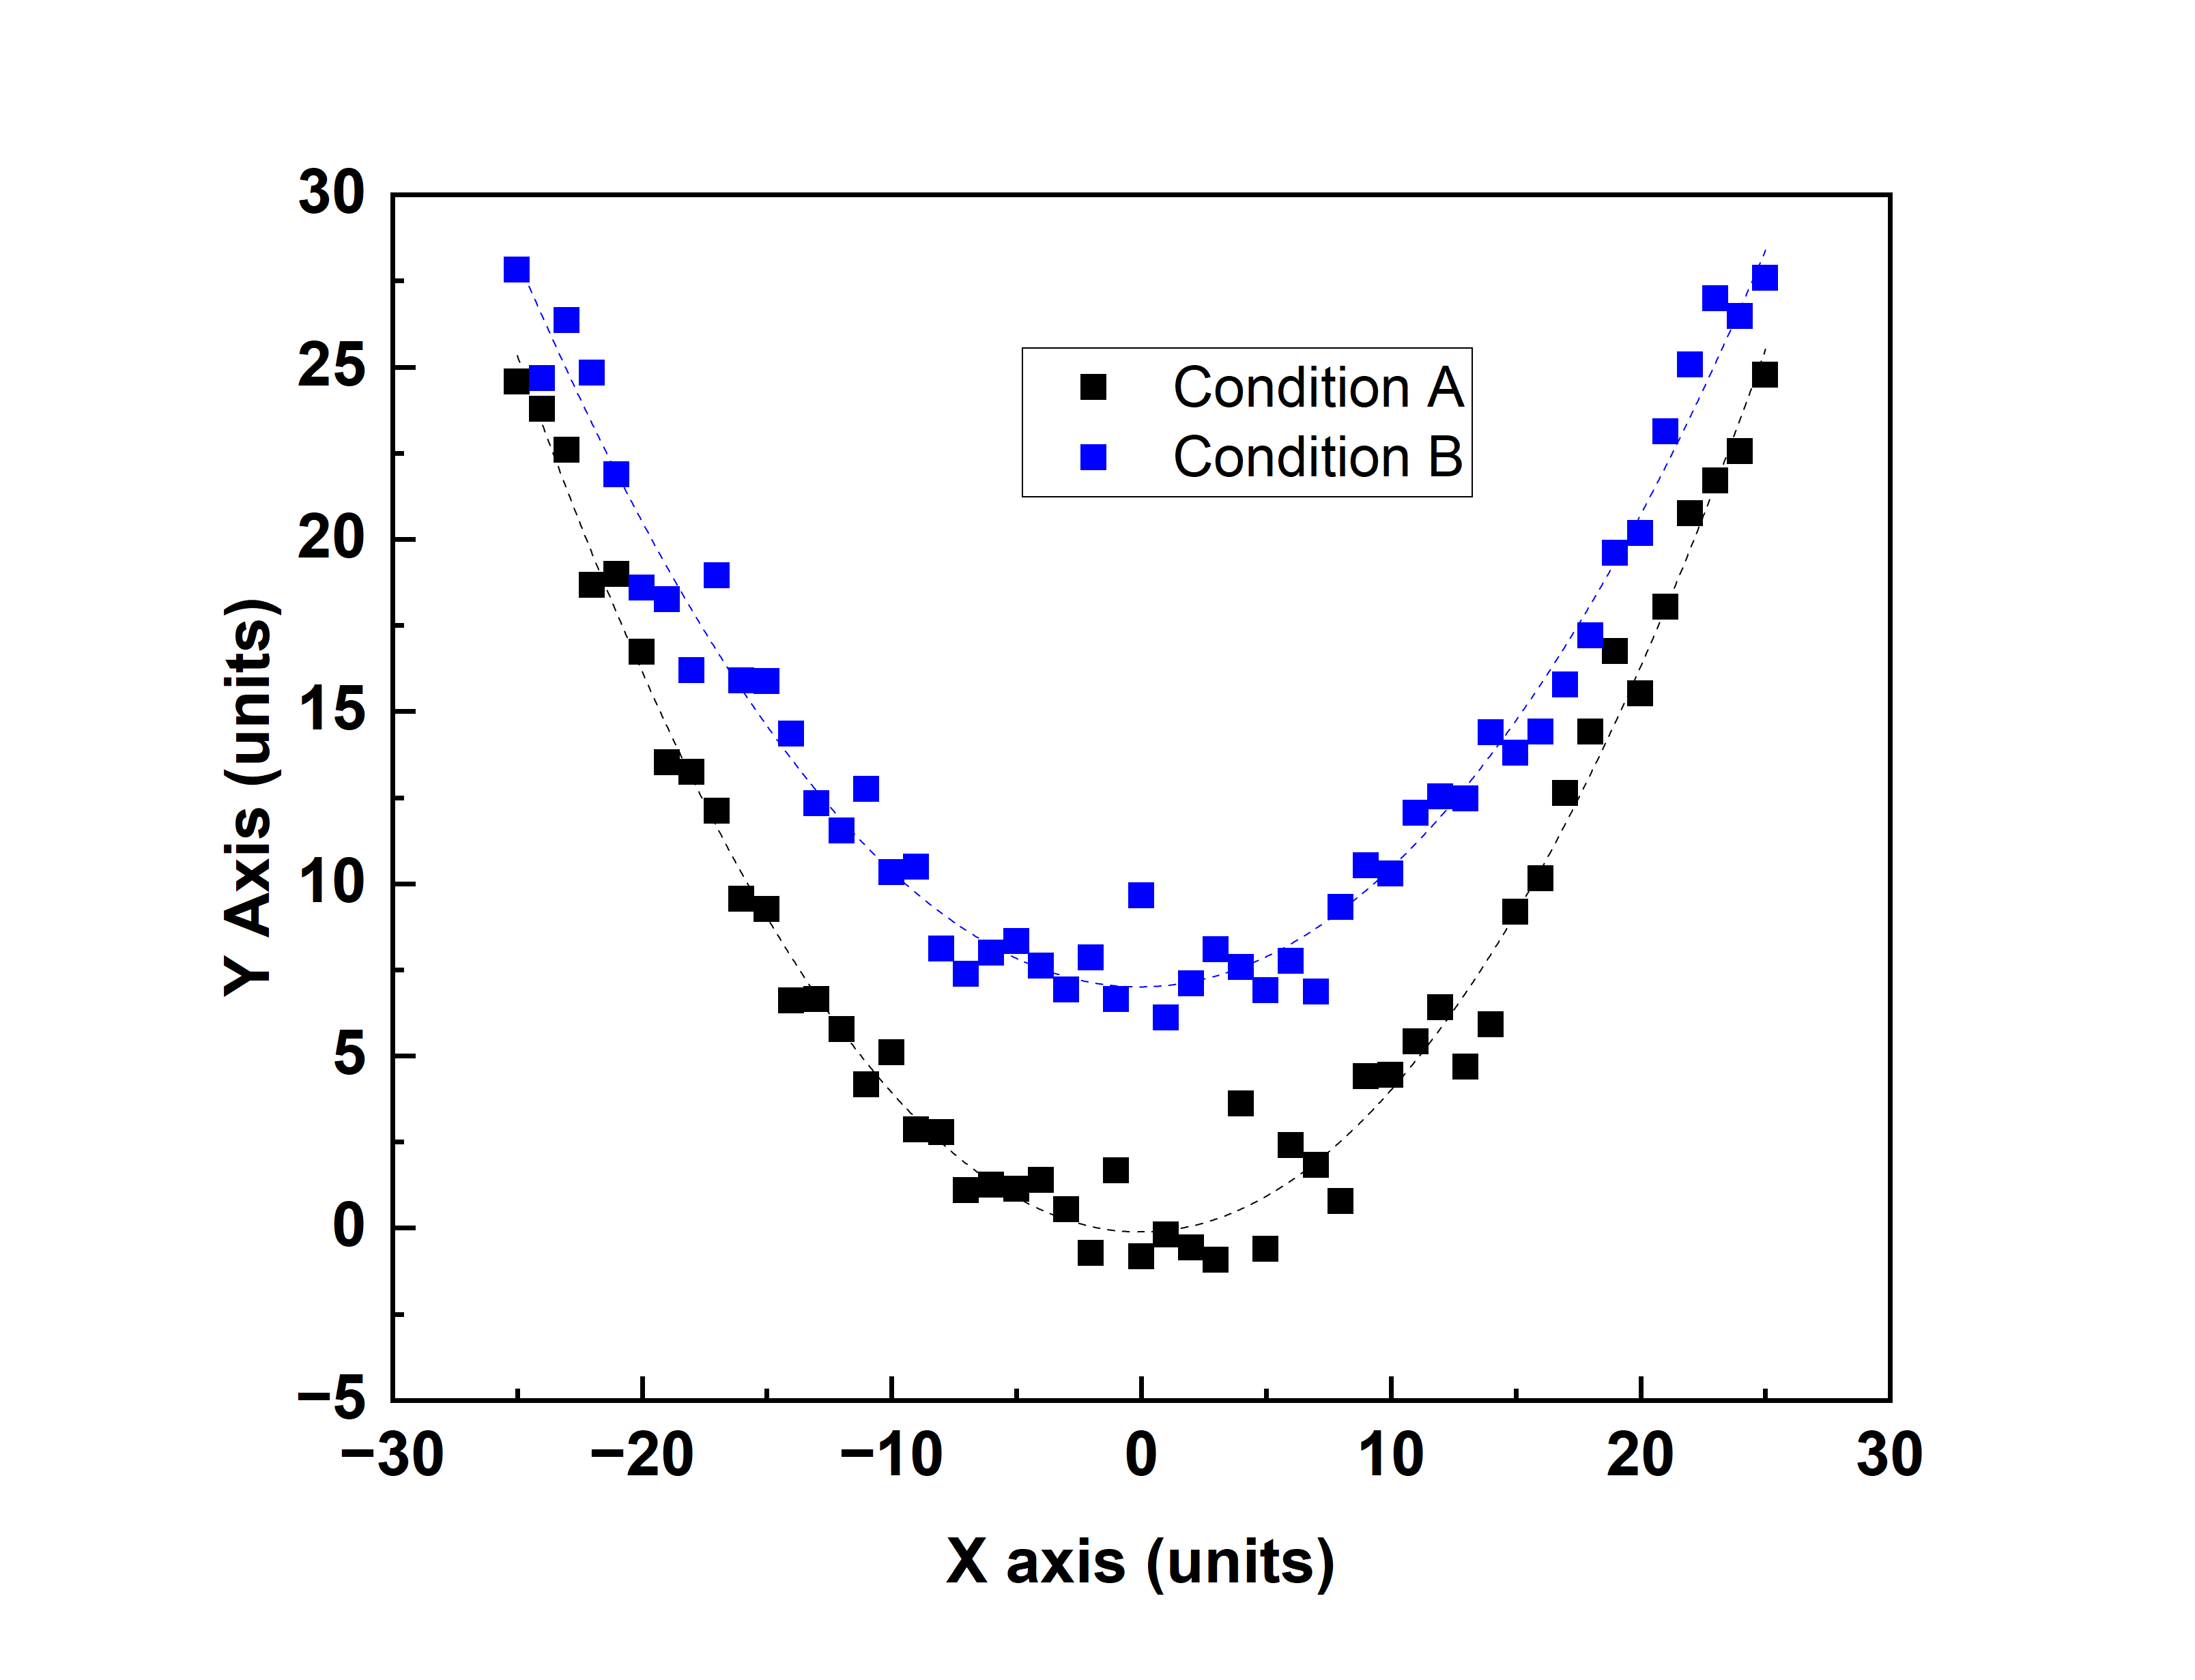
\includegraphics[width=0.75\textwidth]{./images/example}
	\caption[Short title for TOC]{This is a longer caption that actually explains the impact of independent variable X on the response of Y, a critical value that explains the weave quality.}
	\label{fig:sample}
\end{figure}

\begin{table}[htbp]
	\centering
	\caption[Short table title for TOC]{Long table title for content}
	\begin{tabular}{rrr}
	\toprule
	Category & A & B\\
	\midrule
	x & 1 & 2\\
	y & 3 & 4\\
	z & 5 & 6\\
	\bottomrule
	\end{tabular}
	\label{tab:sample}
\end{table}
\chapter{Conclusion}
\appendix
\chapter{Appendix}
This is an appendix.
\backmatter
\cleardoublepage
\phantomsection
\addcontentsline{toc}{chapter}{\bibname}
\bibliography{sample}
\bibliographystyle{rsc}
\end{document}